
\section{TemporalBench}
\label{sec:benchmark}
\begin{figure*}[t]
    \centering
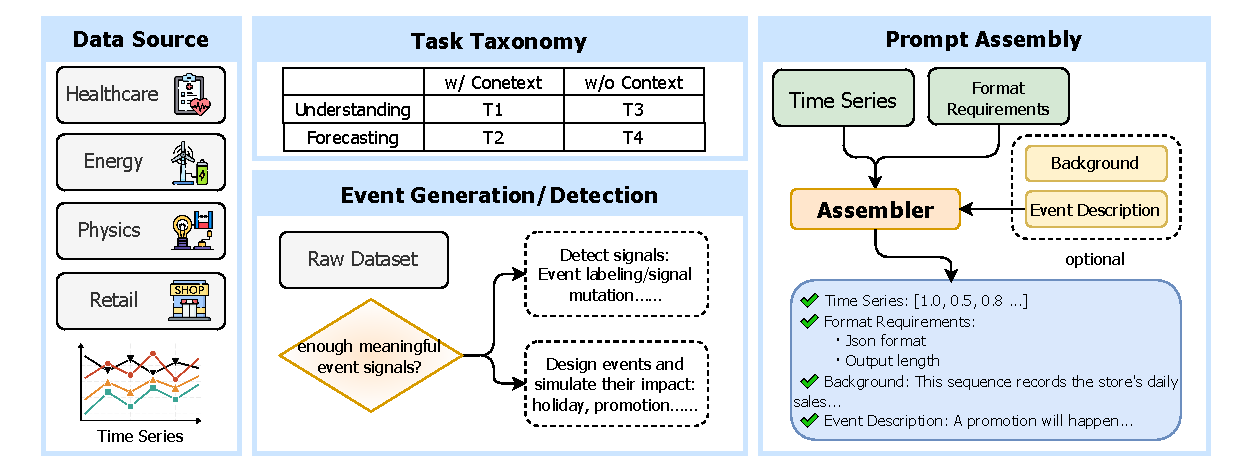
\includegraphics[width=\textwidth]{images/pipeline.pdf}
\vspace{-20pt}
\caption{
Overview of the task generation pipeline in our benchmark, illustrating how raw time-series data are transformed into T1--T4 tasks through event generation or detection, prompt assembly, and format-aware task construction.
}

    \label{fig:pipeline}
\end{figure*}
\subsection{Benchmark Overview}

We introduce \textbf{TemporalBench}, a multi-domain benchmark designed to systematically evaluate agent performance on time-series tasks that require temporal understanding, prediction, and reasoning under contextual and event-driven settings. Rather than treating time-series evaluation as a single forecasting problem, TemporalBench adopts a task-centric design that explicitly probes different temporal competencies through controlled task construction.

TemporalBench is built upon four real-world time-series datasets, spanning retail (\textbf{FreshRetailNet-50K}\cite{wang2025freshretailnet}), healthcare (\textbf{MIMIC-IV}\cite{johnson2023mimic}), energy (\textbf{PSML}\cite{zheng2022multi}), and physical system domains (\textbf{Causal Chambers}\cite{gamella2024causal}). Across these heterogeneous sources, we apply a \emph{unified benchmark construction pipeline} that transforms raw numerical time-series into a structured set of evaluation tasks. An overview of this pipeline is illustrated in Figure~\ref{fig:pipeline}, which shows how event generation or detection, prompt assembly, and format-aware task construction jointly give rise to the four task families (T1–T4).

The resulting benchmark comprises \textbf{2,775} evaluation tasks instantiated over \textbf{191} distinct time-series instances.
For each instance, multiple tasks are generated to probe complementary aspects of temporal intelligence, including intrinsic structure understanding, future prediction, contextual reasoning, and event-informed decision-making.

As summarized in Table~\ref{tab:ts-benchmarks-comparison}, TemporalBench differs from prior temporal and time-series benchmarks by jointly incorporating real numerical time-series signals, explicit contextual information, and reasoning-oriented task formulations across multiple task types.
Tasks are instantiated as either multiple-choice reasoning questions or numerical forecasting objectives, enabling fine-grained analysis of agent behavior across distinct temporal reasoning regimes.

In the following sections, we describe the task taxonomy and benchmark construction pipeline in detail.




\begin{table}[htbp]
%\vspace{-0.3cm}
\centering
\setlength{\tabcolsep}{4pt}
\renewcommand{\arraystretch}{1.1}
\resizebox{\columnwidth}{!}{
\begin{tabular}{lccccc}
\toprule
\textbf{Benchmark} 
& \textbf{TS-Involved} 
& \textbf{Context} 
& \textbf{Reasoning} 
& \textbf{\#Tasks} 
& \textbf{Task Type} \\
\midrule
Test of Time~\cite{fatemi2024test}            
& \ding{55} & \ding{55} & \ding{51} & 1 & QA \\
TRAM~\cite{wang2024tram}                      
& \ding{55} & \ding{55} & \ding{51} & 1 & QA \\
\midrule
TSI-Bench~\cite{du2024tsi}                    
& \ding{51} & \ding{55} & \ding{55} & 1 & TS Analysis \\
TSB-AD~\cite{liu2024elephant}                      
& \ding{51} & \ding{55} & \ding{55} & 1 & TS Analysis \\
GIFT-Eval~\cite{aksu2024gifteval}                     
& \ding{51} & \ding{55} & \ding{55} & 1 & TS Analysis \\
TFB~\cite{qiu2024tfb}                         
& \ding{51} & \ding{55} & \ding{55} & 1 & TS Analysis \\
Time-MMD~\cite{liu2024time}                
& \ding{51} & \ding{55} & \ding{55} & 1 & TS Analysis \\
\midrule
CiK~\cite{williams2024context}                
& \ding{51} & \ding{51} & \ding{55} & 1 & TS Analysis \\
TGTSF~\cite{xu2024intervention}                     
& \ding{51} & \ding{51} & \ding{55} & 1 & TS Analysis \\
\midrule
LLM TS Struggle~\cite{merrill2024language}    
& \ding{51} & \ding{55} & \ding{51} & 2 & QA, TS Analysis \\
MTBench~\cite{chen2025mtbench}                
& \ding{51} & \ding{55} & \ding{51} & 3 & QA, TS Analysis \\
ChatTime~\cite{wang2025chattime}                       
& \ding{51} & \ding{55} & \ding{51} & 3 & QA, TS Analysis \\
\midrule
\textbf{\modelname (Ours)}                    
& \ding{51} & \ding{51} & \ding{51} & 4 & QA, TS Analysis \\
\bottomrule
\end{tabular}
}

\caption{
Comparison of TemporalBench  with existing temporal and time-series related benchmarks.
TS-Involved indicates whether real numerical time-series are included.
Context indicates whether external contextual information is explicitly incorporated.
}

\vspace{-0.8cm}
\label{tab:ts-benchmarks-comparison}
\end{table}

% \subsection{Data Source}


\subsection{Task Families}
We organize TemporalBench into four task families (T1--T4) designed to \emph{disentangle distinct temporal competencies}, rather than to incrementally increase task difficulty.
The task taxonomy is structured along two orthogonal dimensions:
(i) whether the task focuses on interpreting historical data or predicting future behavior, and
(ii) whether reasoning is performed without or with contextual and event information.
For each time-series instance, data are partitioned into historical and future segments using a predefined event boundary, and a complete set of tasks spanning all four families is generated.
T1 and T2 operate solely on numerical time-series signals, while T3 and T4 additionally incorporate textual context reflecting realistic application scenarios.
This unified construction enables controlled comparison across temporal reasoning regimes, ensuring that performance differences across task families arise from changes in temporal and contextual reasoning requirements rather than from uncontrolled variation in data or task format.


\paragraph{T1: Historical Time-Series Understanding.}
T1 tasks evaluate whether an agent can correctly interpret the structure and behavior of a time series based solely on historical observations.
Agents are provided with a historical time-series segment and asked multiple-choice questions about intrinsic temporal properties, including trend direction, volatility level, seasonality, and the presence of anomalies.
By isolating historical interpretation from prediction and context, T1 serves as a probe of an agent’s ability to extract and reason about temporal structure itself.

\paragraph{T2: Future Time-Series Prediction without Context.}
T2 tasks focus on predicting the future segment of a time series using historical observations alone.
Agents are required to either produce numerical forecasts or answer multiple-choice questions concerning anticipated trends, volatility changes, or seasonal patterns.
By excluding contextual information, T2 aligns with traditional forecasting settings while enabling direct comparison between numerical accuracy and qualitative expectations.
Importantly, T1 and T2 do not form an increasing difficulty hierarchy; rather, they isolate complementary competencies related to interpreting past structure and extrapolating future behavior from temporal signals alone.

\paragraph{T3: Contextual Reasoning over Time-Series.}
T3 tasks introduce a fundamental shift from pattern interpretation to contextual temporal reasoning.
In addition to historical time-series data, agents are provided with textual context that grounds the series in domain semantics and real-world conditions.
Rather than asking what the series looks like, T3 questions probe whether an agent can explain, compare, and reason about temporal behavior in light of contextual descriptions.

To systematically localize reasoning failures, T3 tasks are constructed along six capability dimensions, which together form a minimal basis set for contextual temporal reasoning:
\textbf{C1 Alignment} (mapping natural-language conditions to temporal fields or windows),
\textbf{C2 Slicing} (comparing temporal segments across periods or states),
\textbf{C3 Difference Judgment} (reasoning about distributional differences),
\textbf{C4 Lag} (identifying delayed or offset effects),
\textbf{C5 Structure} (recognizing higher-level temporal patterns such as peaks and change points), and
\textbf{C6 Interaction Understanding} (reasoning about joint or interaction effects).
For each time-series instance, multiple questions are generated to cover a subset of these dimensions, enabling fine-grained attribution of reasoning errors.

\paragraph{T4: Event-Informed Time-Series Prediction.}
T4 tasks evaluate event-conditioned and counterfactual temporal reasoning by requiring agents to predict how future time-series behavior would change under specified upcoming events.
Along with historical observations, agents receive background information describing the application context and textual descriptions of future events expected to influence the series, such as extreme weather or other domain-specific interventions.
Agents must integrate historical patterns, contextual semantics, and event information to produce numerical forecasts or qualitative judgments about future trends, volatility, or seasonality.
T4 therefore probes whether temporal information can be reused for conditional reasoning, rather than merely extrapolated under unchanged assumptions.

\paragraph{Diagnostic Role.}
Together, T1–T4 enable TemporalBench to separate numerical prediction from temporal interpretation, and to further test whether temporal information can be aligned with context and used for reasoning under changing conditions.
This decomposition allows experimental results to be traced back to specific temporal competencies, a property that is essential for diagnosing failure modes in agentic time-series systems.




\subsection{Dataset Transformation Pipeline}

We construct TemporalBench through a unified dataset transformation pipeline designed to ensure methodological consistency, reproducibility, and comparability across heterogeneous time-series domains. The pipeline consists of two key components: (i) event injection or detection to define historical–future boundaries, and (ii) ground truth generation to support systematic evaluation across task families.

\subsubsection{Event Injection and Detection}

Events play a central role in TemporalBench by defining the boundary between historical and future segments of each time series and enabling event-centric task construction.
However, the four datasets in our benchmark differ substantially in how events are recorded or manifested.
Some datasets contain dense temporal measurements with sparse or unreliable event annotations, while others naturally exhibit explicit events or intervention signals.

To accommodate this heterogeneity within a unified benchmark design, we adopt two complementary strategies: \emph{event injection} and \emph{event detection}.
The goal of event injection is not to faithfully simulate real-world causal mechanisms, but to introduce controlled and interpretable regime boundaries that support systematic evaluation of event-aware temporal reasoning.
Accordingly, evaluation focuses on whether agents appropriately condition their predictions and decisions on the presence of an event, rather than on the realism or magnitude of the injected effect.

FreshRetailNet-50K and PSML lack reliable event annotations relative to their dense temporal records.
For these datasets, we inject a salient event at a selected time point and simulate its impact on the subsequent segment.
To reduce bias from imperfect simulation, injected events are designed to be coarse and distinctive, and downstream tasks emphasize qualitative changes between historical and future segments, such as shifts in trend, volatility, or seasonality, rather than precise numerical effects.

In contrast, MIMIC-IV and Causal Chambers naturally support event detection.
MIMIC-IV provides explicit clinical event annotations, including procedures, medication administration, and patient transfers.
Causal Chambers does not include explicit event labels, but interventions in the underlying physical system often induce abrupt changes in observed variables, which we detect as change points.
Under both strategies, each time series is partitioned into a historical segment and a future segment by a well-defined event, enabling consistent task construction across heterogeneous datasets.

\subsubsection{Ground Truth Generation}

Ground truth labels in TemporalBench are generated automatically from time-series data using unified, rule-based procedures, without manual annotation or model-dependent heuristics.
Label generation follows three core principles: independence from contextual descriptions, robustness across heterogeneous domains, and explicit handling of uncertainty.

Across all datasets and task families, labels are computed solely from historical and future time-series segments.
Contextual descriptions and event narratives are used only to define the historical--future split and to condition task prompts, and they do not influence any labeling rule.
This design prevents information leakage from event injection or detection and ensures that models cannot succeed by exploiting prompt structure rather than temporal evidence.

To ensure robustness across domains and scales, we rely on statistically stable estimators, including medians, median absolute deviation (MAD), interquartile range (IQR), and Theil--Sen slopes.
Labels are defined primarily in terms of relative changes rather than absolute values.
When observed effects fail to meet predefined strength or support criteria, we assign \emph{Uncertain} labels instead of forcing unreliable decisions.

Ground truth generation is task-specific.
T1 targets intrinsic properties of historical segments, such as trend, volatility, seasonality, and anomalies, using robust statistics and window-based comparisons.
T2 and T4 focus on future behavior, with numerical ground truth given by observed future values and auxiliary multiple-choice labels describing qualitative changes relative to history.
T3 emphasizes higher-level temporal reasoning over historical data, generating labels for questions involving segment comparisons, lagged responses, and interaction effects, with only statistically reliable instances retained.

Additional implementation details and pseudocode for event injection or detection and ground-truth labeling are provided in Appendix~\ref{app:pseudocode}.
